\chapter{Systembeskrivelse} \label{ch:Systembeskrivelse}
Systemet består samlet af en PC, en Xbox-360 controller og en legetøjsbil som styres fra PC'en. Legetøjsbilen styres via et netværk som kræver at både PC og bil er logget på samme router. Bilen tilkobles en trådløs forbindelse hvorimod PC sagtens kan tilgå netværket via kabel. Bilen er udstyret med et antikollisions system som i resten af rapporten er forkortet til AKS. AKS systemet overtager styringen fra brugeren når bilen styres imod en forhindring, således bilen selv kan manøvrere udenom forhindringen. Når brugeren styrer bilen via PC'en er der installerer et GUI hvori der modtages video-stream fra et kamera påmonteret bilen. Endvidere modtages der data fra bilen således brugeren kan se den nuværende hastighed, acceleration og afstand til forhindring. 

\begin{figure}[H]
\centering
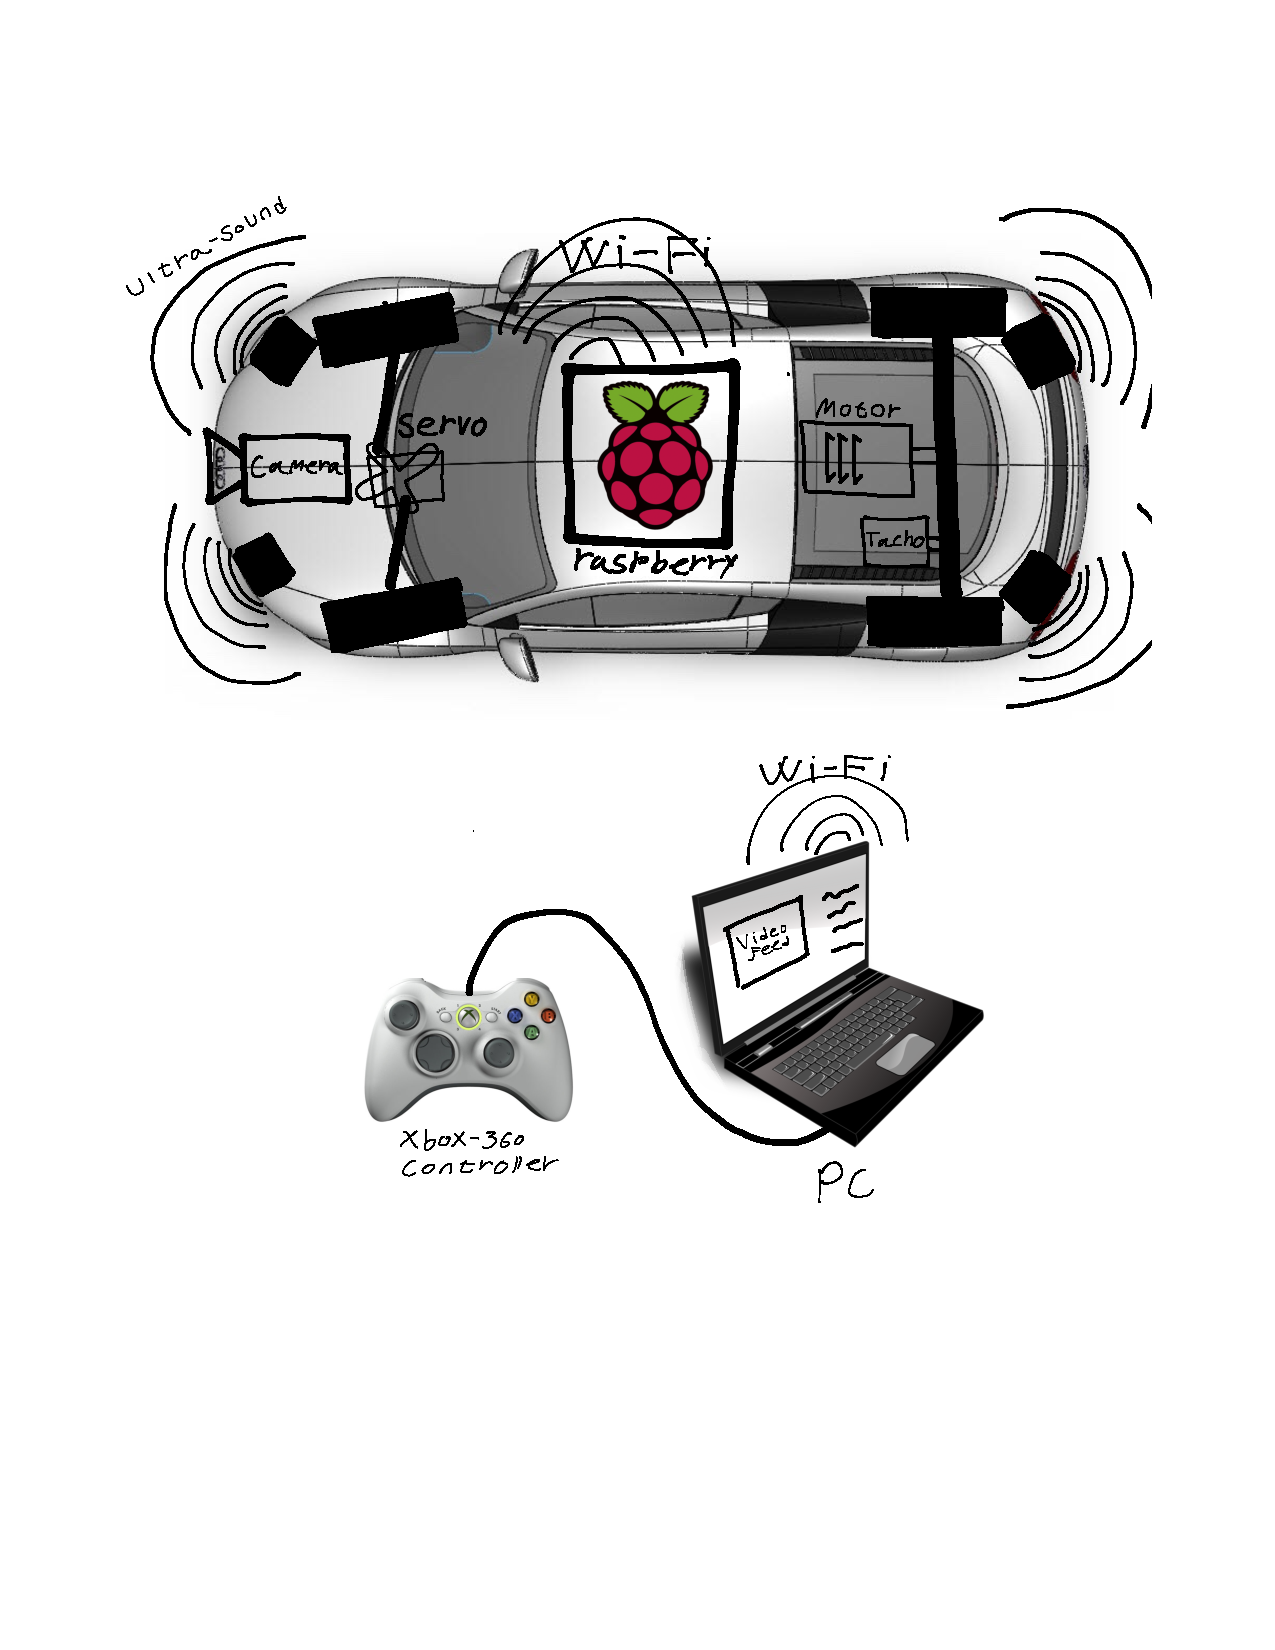
\includegraphics[width=\textwidth - 7.38 cm]{../fig/billeder/rigbillede}
\caption{Rigt billede af systemet i sin helhed}
\label{fig:rigbillede}
\end{figure} 

\begin{figure}[h]
\centering
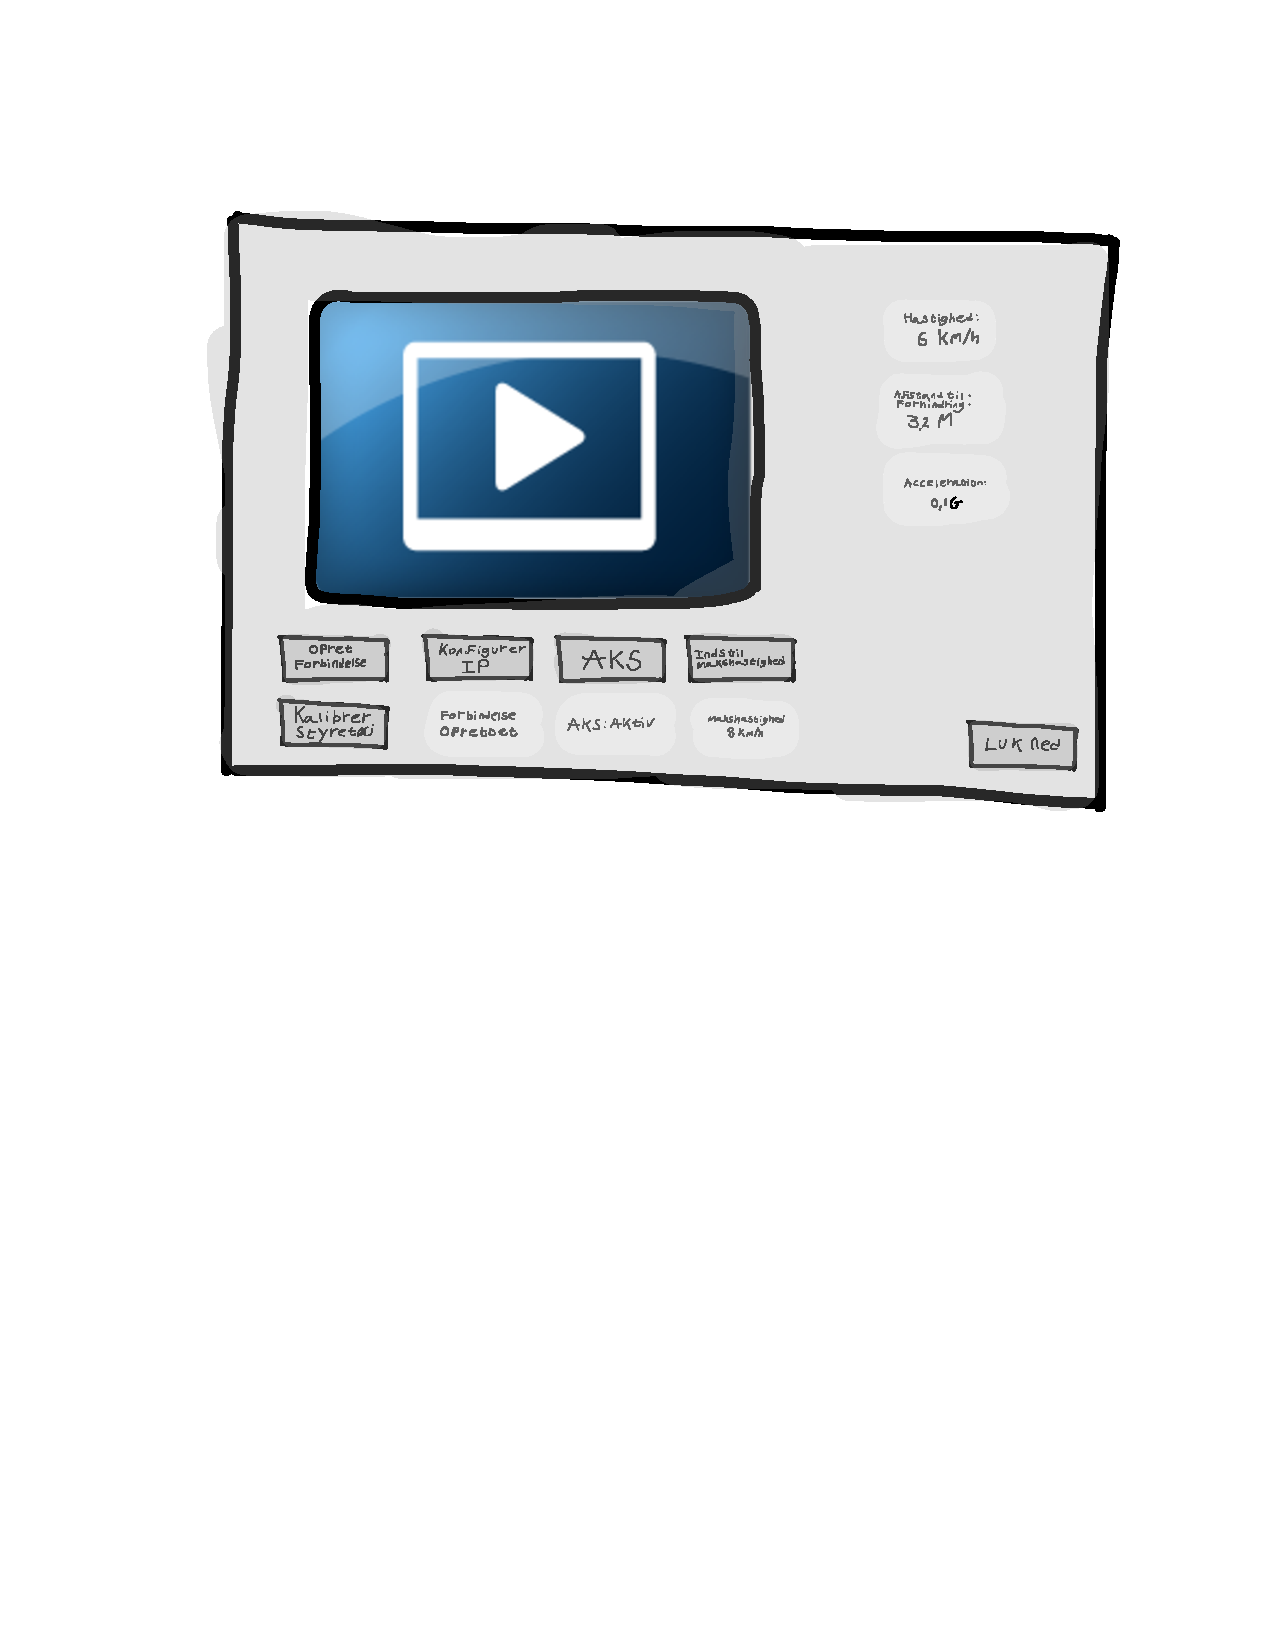
\includegraphics[width=\textwidth*2/3]{../fig/gui/hovedmenu}
\caption{Skitse af hovedmenu}
\label{fig:main_menu}
\end{figure}
